% Provenance (never printed): see sources/outline_sources.md (Year 1: optical
% mineralogy with the polarising microscope; Michel-Levy chart). Interference
% colours in figdata/bachelor-1/michel_levy.py from the CIE 1931 colour-matching
% functions and illuminant D65 (data/derived/bachelor-1-cie*.csv); exercise and
% problem values in the Book 3 scratch calculator calc/ch08.py.
\chapter{Mineralogia óptica}\label{ch:b1:optical-mineralogy}

Entre \omterm{def:b1:field-lab-methods-1:microscope}{polarizadores cruzados}, uma \omterm{def:b1:field-lab-methods-1:thin-section}{lâmina delgada} de gabro acende como um vitral. Ripas longas, cinzentas e brancas, listradas como um código de barras, atravessam o campo; entre elas, grãos brilham em azul, amarelo e magenta; alguns poucos permanecem pretos, qualquer que seja o ângulo. Cada um desses efeitos tem uma causa que pode ser calculada, e cada um indica qual \omterm{def:b1:rock-forming-minerals:mineral}{mineral} está ali. Este capítulo explica como a luz atravessa um cristal, por que um \omterm{def:b1:rock-forming-minerals:mineral}{mineral} entre \omterm{def:b1:field-lab-methods-1:microscope}{polarizadores cruzados} é colorido, como a cor mede uma propriedade do \omterm{def:b1:rock-forming-minerals:mineral}{mineral} e como um petrólogo dá nome aos grãos de uma \omterm{def:b1:field-lab-methods-1:thin-section}{lâmina delgada} usando apenas um microscópio. Ele termina com uma lâmina desconhecida cujos \omterm{def:b1:rock-forming-minerals:mineral}{minerais}, e cuja \omterm{def:b1:cross-sections:thickness}{espessura verdadeira}, são encontrados a partir do que ela mostra.

\begin{recall}
Uma \omterm{def:b1:field-lab-methods-1:thin-section}{lâmina delgada} é uma fatia de rocha com cerca de \qty{30}{\micro m} de espessura sobre uma lâmina de vidro; o \omterm{def:b1:field-lab-methods-1:microscope}{microscópio de polarização} a observa em \omterm{def:b1:field-lab-methods-1:microscope}{luz plano-polarizada} (um polarizador) e entre \omterm{def:b1:field-lab-methods-1:microscope}{polarizadores cruzados} (\cref{ch:b1:field-lab-methods-1}). O índice de refração $n$ de um meio é a razão entre a velocidade da luz no vácuo e a sua velocidade no meio, e a refração em uma interface obedece à lei de Snell $n_1\sin i_1 = n_2\sin i_2$ (física, primeiro ano universitário). A luz é uma onda transversal; um polarizador deixa passar apenas a componente do campo elétrico ao longo da sua direção, de modo que um analisador a um ângulo $\alpha$ deixa passar a fração $\cos^2\alpha$ da intensidade (lei de Malus, física).
\end{recall}

\section{A luz nos cristais}

Em um vidro, um líquido ou um cristal cúbico, a luz viaja com a mesma velocidade em todas as direções e qualquer que seja a sua direção de vibração. Na maioria dos \omterm{def:b1:rock-forming-minerals:mineral}{minerais} não é assim: o arranjo dos átomos difere segundo as diferentes direções, e assim também a resposta dos elétrons ao campo elétrico da onda.

\begin{definition}[Minerais isotrópicos e anisotrópicos]\label{def:b1:optical-mineralogy:anisotropic}
Um \omterm{def:b1:rock-forming-minerals:mineral}{mineral} é um \emph{mineral isotrópico}\index{mineral isotrópico} quando o seu índice de refração é o mesmo para toda direção de propagação e de vibração da luz; \omterm{def:b1:rock-forming-minerals:mineral}{minerais} cúbicos (\omterm{def:b1:rock-forming-minerals:groups}{granada}, halita, espinélio) e vidros são isotrópicos. Ele é um \emph{mineral anisotrópico}\index{mineral anisotrópico} quando o seu índice de refração depende da direção de vibração; todos os \omterm{def:b1:rock-forming-minerals:mineral}{minerais} dos outros sistemas cristalinos são anisotrópicos.
\end{definition}

Uma lâmina cortada de um cristal anisotrópico não deixa a luz passar como uma única onda. Admitimos o seguinte resultado da óptica cristalina (física, segundo ano universitário): para uma dada direção de propagação, uma lâmina de um \omterm{def:b1:optical-mineralogy:anisotropic}{mineral anisotrópico} transmite duas ondas que vibram em duas direções perpendiculares fixas na lâmina, as suas \emph{direções de vibração}, e viajam com dois índices de refração diferentes, $n_1$ e $n_2$. A luz que vibra ao longo de uma dessas direções atravessa a lâmina sem mudar de polarização; a luz que vibra em qualquer outra direção é decomposta nas suas duas componentes ao longo delas. Os dois índices dependem da direção de propagação, e há direções particulares em que eles são iguais.

\begin{definition}[Eixo óptico, minerais uniaxiais e biaxiais]\label{def:b1:optical-mineralogy:optic-axis}
Um \emph{eixo óptico}\index{eixo óptico} de um \omterm{def:b1:optical-mineralogy:anisotropic}{mineral anisotrópico} é uma direção de propagação ao longo da qual a luz viaja com um único índice de refração, qualquer que seja a sua direção de vibração, como em um meio isotrópico. Um \omterm{def:b1:rock-forming-minerals:mineral}{mineral} é \emph{uniaxial}\index{uniaxial} quando tem um eixo óptico (\omterm{def:b1:rock-forming-minerals:mineral}{minerais} dos sistemas trigonal, tetragonal e hexagonal, como o quartzo e a calcita), e \emph{biaxial}\index{biaxial} quando tem dois (\omterm{def:b1:rock-forming-minerals:mineral}{minerais} ortorrômbicos, monoclínicos e triclínicos, como a \omterm{def:b1:rock-forming-minerals:groups}{olivina}, os \omterm{def:b1:rock-forming-minerals:groups}{piroxênios}, os \omterm{def:b1:rock-forming-minerals:groups}{anfibólios}, as \omterm{def:b1:rock-forming-minerals:groups}{micas} e os \omterm{def:b1:rock-forming-minerals:groups}{feldspatos}).
\end{definition}

A geometria é resumida por uma superfície, a indicatriz: um elipsoide cujo raio em cada direção é o índice de refração da luz que vibra nessa direção. A seção do elipsoide perpendicular à direção de propagação é uma elipse cujos eixos são as duas direções de vibração e cujos semieixos são $n_1$ e $n_2$. Para um \omterm{def:b1:rock-forming-minerals:mineral}{mineral} \omterm{def:b1:optical-mineralogy:optic-axis}{uniaxial} o elipsoide é de revolução em torno do \omterm{def:b1:optical-mineralogy:optic-axis}{eixo óptico}, com dois índices principais $n_\omega$ e $n_\varepsilon$: o quartzo tem $n_\omega = 1.544$ e $n_\varepsilon = 1.553$, a calcita $1.658$ e $1.486$.
% ledger: hom:quartz-optics, hom:calcite-optics
Um \omterm{def:b1:rock-forming-minerals:mineral}{mineral} \omterm{def:b1:optical-mineralogy:optic-axis}{biaxial} tem três índices principais $n_\alpha < n_\beta < n_\gamma$ e duas seções circulares, perpendiculares aos seus dois \omterm{def:b1:optical-mineralogy:optic-axis}{eixos ópticos}: a forsterita tem $1.635$, $1.651$ e $1.670$.
% ledger: hom:forsterite-optics

\begin{definition}[Birrefringência (de um mineral)]\label{def:b1:optical-mineralogy:birefringence}
A \emph{birrefringência}\index{birrefringência (de um mineral)} de um \omterm{def:b1:rock-forming-minerals:mineral}{mineral} é a diferença $\delta = n_{\max} - n_{\min}$ entre os seus maiores e menores índices de refração principais: $n_\varepsilon - n_\omega$ em valor absoluto para um \omterm{def:b1:rock-forming-minerals:mineral}{mineral} \omterm{def:b1:optical-mineralogy:optic-axis}{uniaxial}, $n_\gamma - n_\alpha$ para um \omterm{def:b1:optical-mineralogy:optic-axis}{biaxial}. Em um grão cortado em qualquer outra direção, a diferença $|n_1 - n_2|$ fica entre 0 (uma seção perpendicular a um \omterm{def:b1:optical-mineralogy:optic-axis}{eixo óptico}) e $\delta$ (uma seção que contém as direções de $n_{\max}$ e $n_{\min}$).
\end{definition}

A \omterm{def:b1:optical-mineralogy:birefringence}{birrefringência} é uma propriedade do \omterm{def:b1:rock-forming-minerals:mineral}{mineral}, como a sua densidade: quartzo \num{0.009}, calcita \num{0.172}, forsterita \num{0.035}, fayalita \num{0.052}. Uma \omterm{def:b1:field-lab-methods-1:thin-section}{lâmina delgada} corta os grãos de um \omterm{def:b1:rock-forming-minerals:mineral}{mineral} em todas as orientações, de modo que os seus grãos mostram todos os valores de 0 a $\delta$; só o mais alto é característico.
% ledger: hom:quartz-optics, hom:calcite-optics, hom:forsterite-optics, hom:fayalite-optics

\section{Observações em luz plano-polarizada}

Com apenas o polarizador inferior, o microscópio mostra a forma dos grãos, a sua cor, as suas clivagens e o seu \omterm{def:b1:optical-mineralogy:relief}{relevo}.

\begin{definition}[Pleocroísmo]\label{def:b1:optical-mineralogy:pleochroism}
Um \omterm{def:b1:rock-forming-minerals:mineral}{mineral} é \emph{pleocroico}\index{pleocroísmo} quando a sua cor, vista em \omterm{def:b1:field-lab-methods-1:microscope}{luz plano-polarizada}, muda à medida que a platina é girada; o \emph{pleocroísmo} é essa mudança. Ele surge porque a absorção da luz depende da sua direção de vibração no cristal.
\end{definition}

A biotita é o caso clássico: um grão cortado transversalmente à sua clivagem passa de marrom-amarelado pálido a marrom escuro à medida que gira, mais escuro quando os traços da clivagem ficam ao longo do polarizador. A hornblenda muda de amarelo para verde. A maioria dos outros silicatos formadores de rochas (quartzo, \omterm{def:b1:rock-forming-minerals:groups}{feldspatos}, \omterm{def:b1:rock-forming-minerals:groups}{olivina}, diopsídio, muscovita) é incolor em \omterm{def:b1:field-lab-methods-1:thin-section}{lâmina delgada}, e os seus grãos incolores são distinguidos por outros meios.
% ledger: hom:biotite-optics, hom:hornblende-optics, hom:muscovite-optics, hom:diopside-optics, hom:forsterite-optics

\begin{definition}[Relevo, linha de Becke]\label{def:b1:optical-mineralogy:relief}
O \emph{relevo}\index{relevo (óptico)} de um grão em \omterm{def:b1:field-lab-methods-1:thin-section}{lâmina delgada} é o quanto o seu contorno, suas fissuras e sua superfície se destacam contra o meio de montagem; ele é alto quando os índices de refração do grão e do meio diferem muito, baixo quando estão próximos. A \emph{linha de Becke}\index{linha de Becke} é a fina linha brilhante que borda um grão cujo índice difere do de seus arredores quando o microscópio está levemente fora de foco.
\end{definition}

\begin{proposition}[Relevo e índice de refração]\label{prop:b1:optical-mineralogy:relief}
Um raio que atravessa com incidência $i$ uma fronteira entre um meio de montagem de índice
$n_m$ e um grão de índice $n$ próximo de $n_m$ é desviado de
\[
  \varepsilon \approx \frac{|n - n_m|}{n_m}\,\tan i
\]
(em radianos), até primeira \omterm{def:b1:optical-mineralogy:interference-colour}{ordem} em $(n - n_m)/n_m$. Os desvios nas bordas inclinadas de um grão, e assim o seu \omterm{def:b1:optical-mineralogy:relief}{relevo}, crescem em proporção a
$|n - n_m|$.
\end{proposition}

\begin{proof}
A lei de Snell dá $n_m \sin i = n \sin r$. Escreva $n = n_m(1 + \eta)$ com
$\eta$ pequeno e $r = i - \varepsilon$ com $\varepsilon$ pequeno. Então
$\sin i = (1 + \eta)(\sin i - \varepsilon\cos i) + O(\eta^2, \varepsilon^2)$,
logo $\eta \sin i = \varepsilon\cos i$ até primeira \omterm{def:b1:optical-mineralogy:interference-colour}{ordem}, isto é,
$\varepsilon = \eta\tan i$, com $|\eta| = |n - n_m|/n_m$.
\end{proof}

Uma \omterm{def:b1:field-lab-methods-1:thin-section}{lâmina delgada} é montada em uma resina de índice de cerca de $1.54$.
% ledger: jaic:epoxy-ri
O quartzo ($1.544$--$1.553$) e os \omterm{def:b1:rock-forming-minerals:groups}{feldspatos} ($1.52$--$1.59$) são quase invisíveis contra ela: \omterm{def:b1:optical-mineralogy:relief}{relevo} baixo, bordas dos grãos difíceis de ver. A \omterm{def:b1:rock-forming-minerals:groups}{olivina} ($1.64$--$1.88$), os \omterm{def:b1:rock-forming-minerals:groups}{piroxênios} e os \omterm{def:b1:rock-forming-minerals:groups}{anfibólios} se destacam com bordas escuras e uma superfície de aspecto áspero: \omterm{def:b1:optical-mineralogy:relief}{relevo} alto. A \omterm{def:b1:rock-forming-minerals:groups}{granada} ($1.83$) parece quase cercada de preto. A calcita, cujo índice vai de $1.486$ a $1.658$ conforme a direção de vibração, muda de \omterm{def:b1:optical-mineralogy:relief}{relevo} à medida que a platina gira, um efeito chamado cintilação.
% ledger: hom:quartz-optics, hom:albite-optics, hom:anorthite-optics, hom:orthoclase-optics, hom:forsterite-optics, hom:fayalite-optics, hom:almandine-optics, hom:calcite-optics
O \omterm{def:b1:optical-mineralogy:relief}{relevo} indica apenas o quanto $n$ difere de $n_m$, e não de que lado; a \omterm{def:b1:optical-mineralogy:relief}{linha de Becke} indica o lado.

\begin{method}[O teste da linha de Becke]\label{met:b1:optical-mineralogy:becke}
Focalize a borda de um grão em \omterm{def:b1:field-lab-methods-1:microscope}{luz plano-polarizada}, feche um pouco o diafragma de abertura e eleve levemente o foco (afaste a objetiva da seção). A \omterm{def:b1:optical-mineralogy:relief}{linha de Becke} brilhante se desloca para o meio de maior índice de refração: se ela se desloca para dentro do grão, o grão tem o índice mais alto (\omterm{def:b1:optical-mineralogy:relief}{relevo} positivo); se ela se desloca para fora, para a montagem ou para o grão vizinho, o grão tem o índice mais baixo (\omterm{def:b1:optical-mineralogy:relief}{relevo} negativo).
\end{method}

O método funciona porque uma borda de grão nunca é exatamente vertical: em uma borda inclinada, a luz é refratada na direção do lado de maior índice, e além do ângulo crítico ela é totalmente refletida desse lado, de modo que a luz que atravessa a borda se concentra acima do meio de maior índice. Elevar o foco olha para um plano acima da seção, onde essa luz concentrada está dentro do material de maior índice.

\section{Entre polarizadores cruzados}

Com o analisador inserido, em ângulo reto com o polarizador, um grão isotrópico é preto em todas as posições: a luz o alcança vibrando ao longo do polarizador e sai dele vibrando do mesmo modo, e o analisador a barra inteiramente. Um grão anisotrópico é em geral brilhante e colorido. A razão é o atraso entre as suas duas ondas.

\begin{definition}[Retardo (em uma lâmina cristalina)]\label{def:b1:optical-mineralogy:retardation}
O \emph{retardo}\index{retardo (em uma lâmina cristalina)} $\Delta$ de uma lâmina de um \omterm{def:b1:optical-mineralogy:anisotropic}{mineral anisotrópico} é a diferença entre os caminhos ópticos das suas duas ondas ao sair da lâmina, a onda mais lenta ficando atrás da mais rápida.
\end{definition}

\begin{proposition}[Retardo e birrefringência]\label{prop:b1:optical-mineralogy:retardation}
Uma lâmina de espessura $d$ cujas duas ondas têm índices $n_1 > n_2$ tem o \omterm{def:b1:optical-mineralogy:retardation}{retardo}
\[
  \Delta = d\,(n_1 - n_2),
\]
e as suas duas ondas saem com uma diferença de fase $\varphi = 2\pi\Delta/\lambda$ para luz de comprimento de onda $\lambda$ no vácuo. Em uma \omterm{def:b1:field-lab-methods-1:thin-section}{lâmina delgada}, o maior \omterm{def:b1:optical-mineralogy:retardation}{retardo} mostrado pelos grãos de um \omterm{def:b1:rock-forming-minerals:mineral}{mineral} é $d\,\delta$.
\end{proposition}

\begin{proof}
Uma onda que atravessa uma espessura $d$ com velocidade $c/n$ leva o tempo $nd/c$; seu caminho óptico, a distância que a luz percorreria no vácuo nesse tempo, é $nd$. As duas ondas entram juntas; ao sair, a mais lenta está atrás por $n_1 d - n_2 d = d(n_1 - n_2)$, um atraso que é a fração $\Delta/\lambda$ de um período, isto é, uma fase $2\pi\Delta/\lambda$. O maior valor de $n_1 - n_2$ entre todas as orientações é $\delta$ (\cref{def:b1:optical-mineralogy:birefringence}).
\end{proof}

Um grão de quartzo da orientação mais favorável em uma seção de \qty{30}{\micro m} de espessura tem $\Delta = \qty{30000}{nm}\times0.009 =
\qty{270}{nm}$; um grão de calcita, $\qty{30000}{nm}\times0.172 = \qty{5160}{nm}$.

\begin{omfigure}
\begin{tikzpicture}[x=1cm, y=1cm, >={Stealth},
  sub/.style={align=center, font=\small, text width=4.2cm}]
% (a) the polariser
\begin{scope}
  \draw[gray!60] (-1.4,0) -- (1.4,0) (0,-1.4) -- (0,1.4);
  \node[gray, font=\scriptsize] at (1.55,-0.2) {L};
  \node[gray, font=\scriptsize] at (0.2,1.55) {N};
  \draw[very thick, omDef, <->] (-1.2,0) -- (1.2,0);
  \node[omDef, font=\scriptsize, above] at (0.75,0.05) {$E_0$};
  \node[sub] at (0,-2.1) {(a) após o polarizador:\\ vibração leste--oeste};
\end{scope}
% (b) inside the plate
\begin{scope}[shift={(5.0,0)}]
  \draw[gray!60] (-1.4,0) -- (1.4,0) (0,-1.4) -- (0,1.4);
  \draw[omThm, thick] (-1.35*0.866,-1.35*0.5) -- (1.35*0.866,1.35*0.5);
  \draw[omThm, thick] (1.35*0.5,-1.35*0.866) -- (-1.35*0.5,1.35*0.866);
  \node[omThm, font=\scriptsize] at (1.42,0.95) {1};
  \node[omThm, font=\scriptsize] at (-0.85,1.32) {2};
  \draw[very thick, omDef, ->] (0,0) -- (1.2,0);
  \draw[omProp, very thick, ->] (0,0) -- (1.2*0.866*0.866,1.2*0.866*0.5);
  \draw[omProp, very thick, ->] (0,0) -- (1.2*0.5*0.5,-1.2*0.5*0.866);
  \draw[densely dotted] (1.2,0) -- (1.2*0.866*0.866,1.2*0.866*0.5) (1.2,0) -- (1.2*0.5*0.5,-1.2*0.5*0.866);
  \draw (0.55,0) arc[start angle=0, end angle=30, radius=0.55];
  \node[font=\scriptsize] at (0.75,0.17) {$\theta$};
  \node[omProp, font=\scriptsize] at (0.45,1.0) {$E_0\cos\theta$};
  \node[omProp, font=\scriptsize, anchor=east] at (0.1,-0.85) {$E_0\sin\theta$};
  \node[sub] at (0,-2.1) {(b) na lâmina: duas ondas ao longo\\ das direções de vibração 1 e 2};
\end{scope}
% (c) at the analyser
\begin{scope}[shift={(10.0,0)}]
  \draw[gray!60] (-1.4,0) -- (1.4,0);
  \draw[very thick, omMeth, <->] (0,-1.3) -- (0,1.3);
  \node[omMeth, font=\scriptsize, right] at (0.05,1.2) {analisador};
  \draw[omProp, very thick, ->] (0,0) -- (1.2*0.866*0.866,1.2*0.866*0.5);
  \draw[omProp, very thick, ->] (0,0) -- (1.2*0.5*0.5,-1.2*0.5*0.866);
  \draw[densely dotted] (1.2*0.866*0.866,1.2*0.866*0.5) -- (0,1.2*0.866*0.5)
                        (1.2*0.5*0.5,-1.2*0.5*0.866) -- (0,-1.2*0.5*0.866);
  \draw[omMeth, very thick, ->] (0,0) -- (0,1.2*0.866*0.5);
  \draw[omMeth, very thick, ->] (0,0) -- (0,-1.2*0.5*0.866);
  \node[omMeth, font=\scriptsize, anchor=east] at (-0.08,0.52) {$+E_0\sin\theta\cos\theta$};
  \node[omMeth, font=\scriptsize, anchor=east] at (-0.08,-0.52) {$-E_0\sin\theta\cos\theta$};
  \node[sub] at (0,-2.1) {(c) no analisador: cada onda\\ passa a sua componente norte--sul};
\end{scope}
\end{tikzpicture}

{\small Luz através de uma lâmina cristalina entre \omterm{def:b1:field-lab-methods-1:microscope}{polarizadores cruzados}. O polarizador deixa passar a vibração leste--oeste (a); a lâmina a decompõe em duas ondas ao longo das suas direções de vibração, a $\theta$ e $\theta + \ang{90}$ do polarizador (b); o analisador, norte--sul, deixa passar a componente norte--sul de cada uma (c). As duas componentes têm tamanhos iguais e sinais opostos: sem o \omterm{def:b1:optical-mineralogy:retardation}{retardo} elas se anulam, e a lâmina parece escura; a onda 2 fica atrás da onda 1 pela fase $\varphi = 2\pi\Delta/\lambda$, e a soma já não se anula.}
\end{omfigure}

\begin{theorem}[Intensidade entre polarizadores cruzados]\label{thm:b1:optical-mineralogy:intensity}
Uma lâmina de \omterm{def:b1:optical-mineralogy:retardation}{retardo} $\Delta$ cujas direções de vibração fazem o ângulo
$\theta$ com o polarizador, entre \omterm{def:b1:field-lab-methods-1:microscope}{polarizadores cruzados}, transmite no comprimento de onda $\lambda$ a intensidade
\[
  I = I_0\,\sin^2 2\theta\,\sin^2\frac{\pi\Delta}{\lambda},
\]
onde $I_0$ é a intensidade que sai do polarizador.
\end{theorem}

\begin{proof}
Tome o polarizador ao longo de $x$ e o analisador ao longo de $y$, e escreva o campo que sai do polarizador como a parte real de $E_0 e^{i\omega t}$ ao longo de $x$, com
$I_0 = E_0^2$ a menos de uma constante. A direção de vibração 1 da lâmina é o vetor unitário $(\cos\theta, \sin\theta)$, a direção 2 é $(-\sin\theta, \cos\theta)$.
O campo incidente tem as componentes $E_0\cos\theta$ ao longo de 1 e
$-E_0\sin\theta$ ao longo de 2. A lâmina deixa a onda 1 inalterada, a menos de uma fase comum, e atrasa a onda 2 de $\varphi = 2\pi\Delta/\lambda$
(\cref{prop:b1:optical-mineralogy:retardation}); em amplitudes complexas, as ondas que saem da lâmina são $E_0\cos\theta$ ao longo de 1 e
$-E_0\sin\theta\,e^{-i\varphi}$ ao longo de 2. Suas componentes ao longo de $y$ são
$E_0\cos\theta\sin\theta$ e $-E_0\sin\theta\cos\theta\,e^{-i\varphi}$; o analisador deixa passar a soma delas,
\[
  A = E_0\sin\theta\cos\theta\,(1 - e^{-i\varphi}) .
\]
Como $|1 - e^{-i\varphi}|^2 = 2 - 2\cos\varphi = 4\sin^2(\varphi/2)$ e
$\sin\theta\cos\theta = \frac12\sin2\theta$, a intensidade é
$|A|^2 = E_0^2\,\sin^2 2\theta\,\sin^2(\varphi/2)$, isto é,
$I = I_0\sin^2 2\theta\sin^2(\pi\Delta/\lambda)$. Se a onda 1 é a mais lenta, $\varphi$ muda de sinal e $I$ não se altera.
\end{proof}

O teorema contém tudo o que o microscópio mostra entre \omterm{def:b1:field-lab-methods-1:microscope}{polarizadores cruzados}. Seu primeiro fator depende apenas da orientação do grão na platina; o segundo, apenas do \omterm{def:b1:optical-mineralogy:retardation}{retardo} do grão e da cor da luz.

\begin{definition}[Posição de extinção, ângulo de extinção]\label{def:b1:optical-mineralogy:extinction}
Um grão anisotrópico entre \omterm{def:b1:field-lab-methods-1:microscope}{polarizadores cruzados} está em uma \emph{posição de extinção}\index{posição de extinção} quando está escuro porque as suas direções de vibração são paralelas ao polarizador e ao analisador. O \emph{ângulo de extinção}\index{ângulo de extinção} de um grão é o ângulo entre uma direção visível nele (um traço de clivagem, um alongamento, um plano de \omterm{def:b1:optical-mineralogy:twin}{macla}) e a posição de extinção mais próxima, lido na platina graduada.
\end{definition}

O fator $\sin^2 2\theta$ se anula em $\theta = 0$, \ang{90}, \ang{180} e \ang{270}: um grão fica escuro quatro vezes em uma volta completa da platina, e é mais brilhante no meio do caminho, a \ang{45} da extinção (figura abaixo). Um grão com $\Delta = 0$ --- um \omterm{def:b1:optical-mineralogy:anisotropic}{mineral isotrópico}, ou uma seção perpendicular a um \omterm{def:b1:optical-mineralogy:optic-axis}{eixo óptico} --- permanece escuro em toda a volta. O \omterm{def:b1:optical-mineralogy:extinction}{ângulo de extinção} depende da simetria do cristal: um \omterm{def:b1:rock-forming-minerals:mineral}{mineral} cujas direções de vibração estão ligadas às suas clivagens, como nos \omterm{def:b1:rock-forming-minerals:mineral}{minerais} ortorrômbicos, extingue paralelamente a elas (extinção reta); um monoclínico ou triclínico em geral não (extinção inclinada). O maior \omterm{def:b1:optical-mineralogy:extinction}{ângulo de extinção} entre os traços da clivagem e a direção de vibração lenta é cerca de \ang{38} no diopsídio e \ang{15}--\ang{19} na hornblenda, em seções paralelas a $(010)$: uma das maneiras de distinguir um \omterm{def:b1:rock-forming-minerals:groups}{piroxênio} de um \omterm{def:b1:rock-forming-minerals:groups}{anfibólio} em \omterm{def:b1:field-lab-methods-1:thin-section}{lâmina delgada}.
% ledger: hom:diopside-optics, hom:hornblende-optics

\begin{omfigure}
\begin{tikzpicture}
\begin{axis}[width=0.8\linewidth, height=5cm, xmin=0, xmax=360, ymin=0, ymax=1.08,
  xtick={0,45,90,...,360}, ytick={0,0.5,1},
  tick label style={font=\scriptsize}, label style={font=\small},
  xlabel={ângulo da platina $\theta$ a partir de uma posição de extinção (\si{\degree})},
  ylabel={$I/I_0$}, legend style={font=\scriptsize, at={(0.5,1.03)}, anchor=south, legend columns=3,
  draw=none}, legend cell align=left]
\addplot[omThm, thick] table[x=theta, y=I270] {figdata/out/bachelor-1-michel_levy-rotation.dat};
\addplot[omDef, thick, densely dashed] table[x=theta, y=I100] {figdata/out/bachelor-1-michel_levy-rotation.dat};
\addplot[omMeth, thick, densely dotted] table[x=theta, y=I540] {figdata/out/bachelor-1-michel_levy-rotation.dat};
\legend{$\Delta = \qty{270}{nm}$, $\Delta = \qty{100}{nm}$, $\Delta = \qty{540}{nm}$}
\end{axis}
\end{tikzpicture}

{\small A intensidade transmitida por um grão à medida que a platina gira, no comprimento de onda \qty{550}{nm}, para três \omterm{def:b1:optical-mineralogy:retardation}{retardos} (\cref{thm:b1:optical-mineralogy:intensity}). Quatro extinções por volta, quatro máximos a \ang{45} delas; o \omterm{def:b1:optical-mineralogy:retardation}{retardo} fixa a altura dos máximos, que é quase nula quando $\Delta$ está próximo de um número inteiro de comprimentos de onda.}
\end{omfigure}

\subsection{Cores de interferência}

Em luz branca, o segundo fator $\sin^2(\pi\Delta/\lambda)$ age como um filtro que depende do comprimento de onda. Um grão com $\Delta = \qty{270}{nm}$ deixa passar quase todo o verde e o amarelo ($\lambda$ perto de $2\Delta = 540$\,nm, onde o fator vale 1) e um pouco menos do violeta e do vermelho: parece branco. Um grão com $\Delta = \qty{550}{nm}$ suprime o amarelo-verde ($\lambda = \Delta$) e deixa passar vermelho e azul: parece magenta. À medida que $\Delta$ cresce, os comprimentos de onda suprimidos percorrem o espectro e outros aparecem, e a cor percorre uma sequência fixa.

\begin{definition}[Cor de interferência, ordem, carta de Michel-Lévy]\label{def:b1:optical-mineralogy:interference-colour}
A \emph{cor de interferência}\index{cor de interferência} de um grão anisotrópico é a sua cor entre \omterm{def:b1:field-lab-methods-1:microscope}{polarizadores cruzados} em luz branca, a \ang{45} da extinção; ela depende apenas do seu \omterm{def:b1:optical-mineralogy:retardation}{retardo} $\Delta$. As cores se repetem em faixas de cerca de \qty{550}{nm} de \omterm{def:b1:optical-mineralogy:retardation}{retardo}, cada uma terminando com um matiz vermelho-violeta; cada faixa é uma \emph{ordem}\index{ordem (de uma cor de interferência)} (primeira, segunda, terceira\dots). A \emph{carta de Michel-Lévy}\index{carta de Michel-Lévy} mostra as cores de interferência em função do \omterm{def:b1:optical-mineralogy:retardation}{retardo}, com as retas $\Delta = d\,\delta$ que relacionam a espessura de uma seção, a \omterm{def:b1:optical-mineralogy:birefringence}{birrefringência} de um \omterm{def:b1:rock-forming-minerals:mineral}{mineral} e a sua cor.
\end{definition}

\begin{omfigure}
\begin{tikzpicture}
\begin{axis}[width=0.84\linewidth, height=7.2cm, view={0}{90}, xmin=0, xmax=1800, ymin=0, ymax=50,
  xtick={0,200,...,1800}, ytick={0,10,...,50}, axis on top, clip=false,
  tick label style={font=\scriptsize}, label style={font=\small},
  xlabel={retardo $\Delta$ (nm)}, ylabel={espessura $d$ (\si{\micro m})},
  unbounded coords=jump]
\addplot3[surf, shader=flat corner, mesh/cols=361, mesh/color input=explicit mathparse,
  point meta={symbolic={\thisrow{r},\thisrow{g},\thisrow{b}}}]
  table[x=delta, y=d, z expr=0] {figdata/out/bachelor-1-michel_levy-chart.dat};
\addplot3[black, thin] table[x=x, y=y, z expr=0] {figdata/out/bachelor-1-michel_levy-segments.dat};
\addplot3[white, very thick, densely dashed] coordinates {(0,30,0) (1800,30,0)};
\node[font=\tiny, anchor=south west, rotate=60] at (axis cs:250,50.3,0) {ortoclásio 0.005};
\node[font=\tiny, anchor=south west, rotate=60] at (axis cs:450,50.3,0) {quartzo 0.009};
\node[font=\tiny, anchor=south west, rotate=60] at (axis cs:600,50.3,0) {plagioclásio 0.012};
\node[font=\tiny, anchor=south west, rotate=60] at (axis cs:1000,50.3,0) {hornblenda 0.020};
\node[font=\tiny, anchor=south west, rotate=60] at (axis cs:1500,50.3,0) {diopsídio 0.030};
\node[font=\tiny, anchor=south west, rotate=60] at (axis cs:1750,50.3,0) {forsterita 0.035};
\node[font=\tiny, anchor=west] at (axis cs:1810,45,0) {muscovita 0.040};
\node[font=\tiny, anchor=west] at (axis cs:1810,34.6,0) {fayalita 0.052};
\node[font=\tiny, anchor=west] at (axis cs:1810,10.5,0) {calcita 0.172};
\node[font=\tiny, anchor=west] at (axis cs:1810,30,0) {\qty{30}{\micro m}};
\node[font=\scriptsize, anchor=north] at (axis cs:270,-7,0) {primeira ordem};
\node[font=\scriptsize, anchor=north] at (axis cs:808,-7,0) {segunda ordem};
\node[font=\scriptsize, anchor=north] at (axis cs:1340,-7,0) {terceira ordem};
\end{axis}
\end{tikzpicture}

{\small Uma \omterm{def:b1:optical-mineralogy:interference-colour}{carta de Michel-Lévy} calculada a partir de primeiros princípios: para cada \omterm{def:b1:optical-mineralogy:retardation}{retardo}, a cor da luz branca (iluminante padrão CIE D65) através de \omterm{def:b1:field-lab-methods-1:microscope}{polarizadores cruzados} e de uma lâmina a \ang{45} da extinção, a partir das funções de correspondência de cores CIE 1931 (dados \textcopyright{} CIE, CC BY-SA 4.0) e da transformação sRGB, normalizada à luz transmitida por polarizadores paralelos. As linhas pretas dão $\Delta = d\,\delta$ para a \omterm{def:b1:optical-mineralogy:birefringence}{birrefringência} de cada \omterm{def:b1:rock-forming-minerals:mineral}{mineral}; a linha tracejada é a espessura padrão de \qty{30}{\micro m}. Os matizes vermelho-violeta que encerram as ordens caem em 542, 1074 e \qty{1605}{nm} neste cálculo.}
% ledger: data:b3-cie1931, data:b3-cie-d65, w3c:srgb, hom:orthoclase-optics, hom:quartz-optics, hom:albite-optics, hom:anorthite-optics, hom:hornblende-optics, hom:diopside-optics, hom:forsterite-optics, hom:muscovite-optics, hom:fayalite-optics, hom:calcite-optics
\end{omfigure}

O gráfico é calculado exatamente como diz o teorema. Para cada \omterm{def:b1:optical-mineralogy:retardation}{retardo}, cada comprimento de onda da luz é ponderado por $\sin^2(\pi\Delta/\lambda)$; o espectro transmitido é então convertido em uma cor como o olho a vê, pelas funções padrão de correspondência de cores da colorimetria, e no vermelho, verde e azul de uma tela ou impressora pela transformação sRGB. Três características são
dignas de nota. A primeira \omterm{def:b1:optical-mineralogy:interference-colour}{ordem} começa preta, passa pelo cinza e pelo branco (o único branco da carta fica perto de \qty{270}{nm}, onde o espectro é quase inteiramente transmitido), depois amarelo, laranja e vermelho. A segunda e a terceira ordens são as mais brilhantes, com azul, verde, amarelo e magenta vivos. Além da quarta \omterm{def:b1:optical-mineralogy:interference-colour}{ordem} as cores se desbotam: quando $\Delta$ tem muitos comprimentos de onda, o filtro $\sin^2(\pi\Delta/\lambda)$ oscila várias vezes através do espectro visível, deixa passar cada cor por sua vez e, em média, metade da luz: o grão parece cinza rosado ou esverdeado pálido, o branco de \omterm{def:b1:optical-mineralogy:interference-colour}{ordem} alta da calcita.

Ler a carta é o núcleo da mineralogia óptica. Em uma seção de espessura conhecida, a cor mais alta mostrada por um \omterm{def:b1:rock-forming-minerals:mineral}{mineral} dá a sua \omterm{def:b1:optical-mineralogy:birefringence}{birrefringência}: siga a espessura até a cor, depois a reta que passa por esse ponto até a \omterm{def:b1:optical-mineralogy:birefringence}{birrefringência}. Inversamente, um \omterm{def:b1:rock-forming-minerals:mineral}{mineral} de \omterm{def:b1:optical-mineralogy:birefringence}{birrefringência} conhecida dá a espessura: em uma boa seção de \qty{30}{\micro m}, o quartzo nunca mostra mais que um branco de primeira \omterm{def:b1:optical-mineralogy:interference-colour}{ordem} ou o amarelo mais pálido, e uma seção em que o quartzo mostra amarelo ou laranja é espessa demais.

\begin{history}[Auguste Michel-Lévy]
% ledger: annales:michel-levy, annales:michel-levy-director, commons:michel-levy
\begin{minipage}[t]{0.76\linewidth}\vspace{0pt}
Auguste Michel-Lévy (1844--1911), que se tornou diretor do Serviço Geológico da França, esteve entre os primeiros a identificar \omterm{def:b1:rock-forming-minerals:mineral}{minerais} em rochas de modo sistemático com o \omterm{def:b1:field-lab-methods-1:microscope}{microscópio de polarização}. Antes dele, as cores dos \omterm{def:b1:rock-forming-minerals:mineral}{minerais} entre \omterm{def:b1:field-lab-methods-1:microscope}{polarizadores cruzados} eram usadas empiricamente; ele mostrou que o que importa é a \omterm{def:b1:optical-mineralogy:birefringence}{birrefringência} máxima de cada \omterm{def:b1:rock-forming-minerals:mineral}{mineral}, que pode ser medida comparando as cores dos seus grãos com uma cunha de quartzo cujo \omterm{def:b1:optical-mineralogy:retardation}{retardo} cresce de modo constante ao longo do comprimento. Com o seu aluno Alfred Lacroix publicou, em 1888, \emph{Les minéraux des roches}, um manual das propriedades ópticas dos \omterm{def:b1:rock-forming-minerals:mineral}{minerais} formadores de rochas. A carta que leva o seu nome, com cores em função do \omterm{def:b1:optical-mineralogy:retardation}{retardo} e retas de \omterm{def:b1:optical-mineralogy:birefringence}{birrefringência} igual, ainda é a maneira de ler as \omterm{def:b1:optical-mineralogy:interference-colour}{cores de interferência}.
\end{minipage}\hfill
\begin{minipage}[t]{0.2\linewidth}\vspace{0pt}
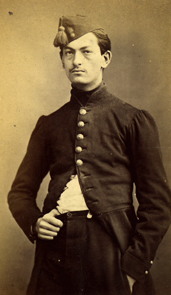
\includegraphics[width=\linewidth]{images/book3/b1-michel-levy.jpg}

{\scriptsize Michel-Lévy como estudante, por volta de 1862. Domínio público.}
\end{minipage}
\end{history}

Duas ondas que saem de um grão podem receber um \omterm{def:b1:optical-mineralogy:retardation}{retardo} extra e conhecido por uma lâmina acessória inserida acima da seção, a \ang{45} dos polarizadores. A mais comum é cortada para mostrar o vermelho de primeira \omterm{def:b1:optical-mineralogy:interference-colour}{ordem}, um \omterm{def:b1:optical-mineralogy:retardation}{retardo} de cerca de \qty{540}{nm}. Se a direção de vibração lenta do grão é paralela à direção lenta da lâmina, os \omterm{def:b1:optical-mineralogy:retardation}{retardos} se somam e a cor do grão sobe de cerca de uma \omterm{def:b1:optical-mineralogy:interference-colour}{ordem}; se ela é paralela à direção rápida, eles se subtraem e a cor desce. Um grão cinza de primeira \omterm{def:b1:optical-mineralogy:interference-colour}{ordem} de \qty{100}{nm} torna-se azul de segunda \omterm{def:b1:optical-mineralogy:interference-colour}{ordem} (\qty{640}{nm}) em uma orientação e laranja de primeira \omterm{def:b1:optical-mineralogy:interference-colour}{ordem} (\qty{440}{nm}) na outra; o teste mostra qual das duas direções de vibração do grão é a lenta, uma propriedade usada para identificar \omterm{def:b1:rock-forming-minerals:mineral}{minerais} alongados.

\section{Identificando minerais em lâmina delgada}

\begin{definition}[Maclagem, maclagem polissintética]\label{def:b1:optical-mineralogy:twin}
Uma \emph{macla}\index{macla (de cristal)} é um crescimento conjunto de dois ou mais cristais do mesmo \omterm{def:b1:rock-forming-minerals:mineral}{mineral} cujas redes se relacionam por uma simetria que o próprio cristal não tem, como uma reflexão em um plano (o plano de macla). A \emph{maclagem polissintética}\index{maclagem polissintética} é uma maclagem repetida em planos paralelos, que divide um cristal em lamelas finas e paralelas cujas orientações se alternam.
\end{definition}

Entre \omterm{def:b1:field-lab-methods-1:microscope}{polarizadores cruzados}, as lamelas de uma \omterm{def:b1:optical-mineralogy:twin}{macla} polissintética se extinguem alternadamente: metade delas está escura quando a outra metade está clara, e o cristal parece listrado. O \omterm{def:b1:rock-forming-minerals:groups}{plagioclásio} quase sempre mostra essas listras, que o distinguem de imediato do quartzo e do \omterm{def:b1:rock-forming-minerals:groups}{feldspato alcalino}; a sua outra característica, o \omterm{def:b1:optical-mineralogy:relief}{relevo} baixo e as cores cinza a branco de primeira \omterm{def:b1:optical-mineralogy:interference-colour}{ordem}, ele compartilha com eles. Os \omterm{def:b1:optical-mineralogy:extinction}{ângulos de extinção} dos dois conjuntos de lamelas, medidos de cada lado do plano de \omterm{def:b1:optical-mineralogy:twin}{macla}, dependem da composição do \omterm{def:b1:rock-forming-minerals:groups}{plagioclásio}, e cartas desses ângulos dão o seu teor de anortita.

\begin{method}[Identificando um mineral em lâmina delgada]\label{met:b1:optical-mineralogy:identify}
\begin{enumerate}
  \item Em \omterm{def:b1:field-lab-methods-1:microscope}{luz plano-polarizada}: observe se o grão é opaco; sua cor e o \omterm{def:b1:optical-mineralogy:pleochroism}{pleocroísmo} (gire a platina); seu \omterm{def:b1:optical-mineralogy:relief}{relevo}, e de que lado de $1.54$ fica o seu índice (\omterm{def:b1:optical-mineralogy:relief}{linha de Becke}); sua forma e suas clivagens, e o ângulo entre duas clivagens.
  \item Entre \omterm{def:b1:field-lab-methods-1:microscope}{polarizadores cruzados}: verifique se ele permanece escuro (isotrópico, ou uma seção perpendicular a um \omterm{def:b1:optical-mineralogy:optic-axis}{eixo óptico}); entre os grãos do mesmo \omterm{def:b1:rock-forming-minerals:mineral}{mineral}, encontre a \omterm{def:b1:optical-mineralogy:interference-colour}{cor de interferência} mais alta e leia a \omterm{def:b1:optical-mineralogy:birefringence}{birrefringência} na \omterm{def:b1:optical-mineralogy:interference-colour}{carta de Michel-Lévy} para a espessura da seção.
  \item Meça o \omterm{def:b1:optical-mineralogy:extinction}{ângulo de extinção} nos grãos que mostram uma clivagem ou um alongamento; procure maclagem (listras polissintéticas, \omterm{def:b1:optical-mineralogy:twin}{maclas} simples).
  \item Compare com uma tabela de propriedades ópticas (\cref{tab:b1:optical-mineralogy:key}) e com os \omterm{def:b1:rock-forming-minerals:mineral}{minerais} que a rocha pode conter (\cref{ch:b1:rock-forming-minerals}).
\end{enumerate}
\end{method}

\begin{table}[htbp]
\centering\footnotesize
\setlength{\tabcolsep}{3pt}
% ledger: hom:quartz-optics, hom:orthoclase-optics, hom:albite-optics, hom:anorthite-optics, hom:muscovite-optics, hom:biotite-optics, hom:hornblende-optics, hom:diopside-optics, hom:forsterite-optics, hom:fayalite-optics, hom:almandine-optics, hom:calcite-optics, hom:magnetite-optics
\begin{tabular}{@{}>{\raggedright\arraybackslash}p{2.0cm}>{\raggedright\arraybackslash}p{2.6cm}>{\raggedright\arraybackslash}p{2.3cm}>{\raggedright\arraybackslash}p{1.8cm}>{\raggedright\arraybackslash}p{3.0cm}>{\raggedright\arraybackslash}p{3.8cm}@{}}
\hline
\omterm{def:b1:rock-forming-minerals:mineral}{mineral} & cor (LPP) & índices & bir\-re\-frin\-gência & cor mais alta a \qty{30}{\micro m} & outras características \\
\hline
quartzo & incolor & 1.544--1.553 & 0.009 & branco de primeira \omterm{def:b1:optical-mineralogy:interference-colour}{ordem} & sem clivagem; sem \omterm{def:b1:optical-mineralogy:twin}{maclas} visíveis; \omterm{def:b1:optical-mineralogy:optic-axis}{uniaxial} \\
ortoclásio & incolor, muitas vezes turvo & 1.518--1.525 & 0.005 & cinza de primeira \omterm{def:b1:optical-mineralogy:interference-colour}{ordem} & \omterm{def:b1:optical-mineralogy:relief}{relevo} negativo; \omterm{def:b1:optical-mineralogy:twin}{maclas} simples \\
\omterm{def:b1:rock-forming-minerals:groups}{plagioclásio} & incolor & 1.526--1.590 & 0.008--0.013 & branco a amarelo pálido de primeira \omterm{def:b1:optical-mineralogy:interference-colour}{ordem} & \omterm{def:b1:optical-mineralogy:twin}{maclagem polissintética} \\
muscovita & incolor & 1.552--1.618 & 0.035--0.042 & brilhante, de segunda a terceira \omterm{def:b1:optical-mineralogy:interference-colour}{ordem} & uma clivagem perfeita; extinção reta \\
biotita & marrom, verde & 1.565--1.696 & 0.04--0.07 & mascarada pela própria cor & forte \omterm{def:b1:optical-mineralogy:pleochroism}{pleocroísmo}; uma clivagem perfeita \\
hornblenda & verde, marrom & 1.675--1.695 & 0.020 & azul de segunda \omterm{def:b1:optical-mineralogy:interference-colour}{ordem} & pleocroica; clivagens a \ang{56}/\ang{124}; extinção \ang{15}--\ang{19} \\
diopsídio & incolor & 1.664--1.694 & 0.030 & amarelo de segunda \omterm{def:b1:optical-mineralogy:interference-colour}{ordem} & clivagens a cerca de \ang{87}/\ang{93}; extinção de cerca de \ang{38} \\
\omterm{def:b1:rock-forming-minerals:groups}{olivina} & incolor (Mg) a amarelo pálido (Fe) & 1.635--1.879 & 0.035--0.052 & do fim da segunda \omterm{def:b1:optical-mineralogy:interference-colour}{ordem} à terceira & \omterm{def:b1:optical-mineralogy:relief}{relevo} alto; fissuras irregulares, sem boa clivagem \\
\omterm{def:b1:rock-forming-minerals:groups}{granada} & incolor a rosa pálido & 1.830 (almandina) & isotrópica & preta & \omterm{def:b1:optical-mineralogy:relief}{relevo} muito alto; contornos de seis ou oito lados \\
calcita & incolor & 1.486--1.658 & 0.172 & branco de \omterm{def:b1:optical-mineralogy:interference-colour}{ordem} alta & o \omterm{def:b1:optical-mineralogy:relief}{relevo} muda na rotação; clivagem romboédrica \\
magnetita & opaca & --- & --- & --- & preta nas duas luzes \\
\hline
\end{tabular}
\caption{Propriedades ópticas de \omterm{def:b1:rock-forming-minerals:mineral}{minerais} formadores de rochas comuns em \omterm{def:b1:field-lab-methods-1:thin-section}{lâmina delgada}.
LPP: \omterm{def:b1:field-lab-methods-1:microscope}{luz plano-polarizada}. A cor mais alta é lida na \omterm{def:b1:optical-mineralogy:interference-colour}{carta de Michel-Lévy} em $\Delta = \qty{30000}{nm}\times\delta$.}
\label{tab:b1:optical-mineralogy:key}
\end{table}

\begin{omfigure}
\setlength{\tabcolsep}{2pt}
\begin{tabular}{cc}
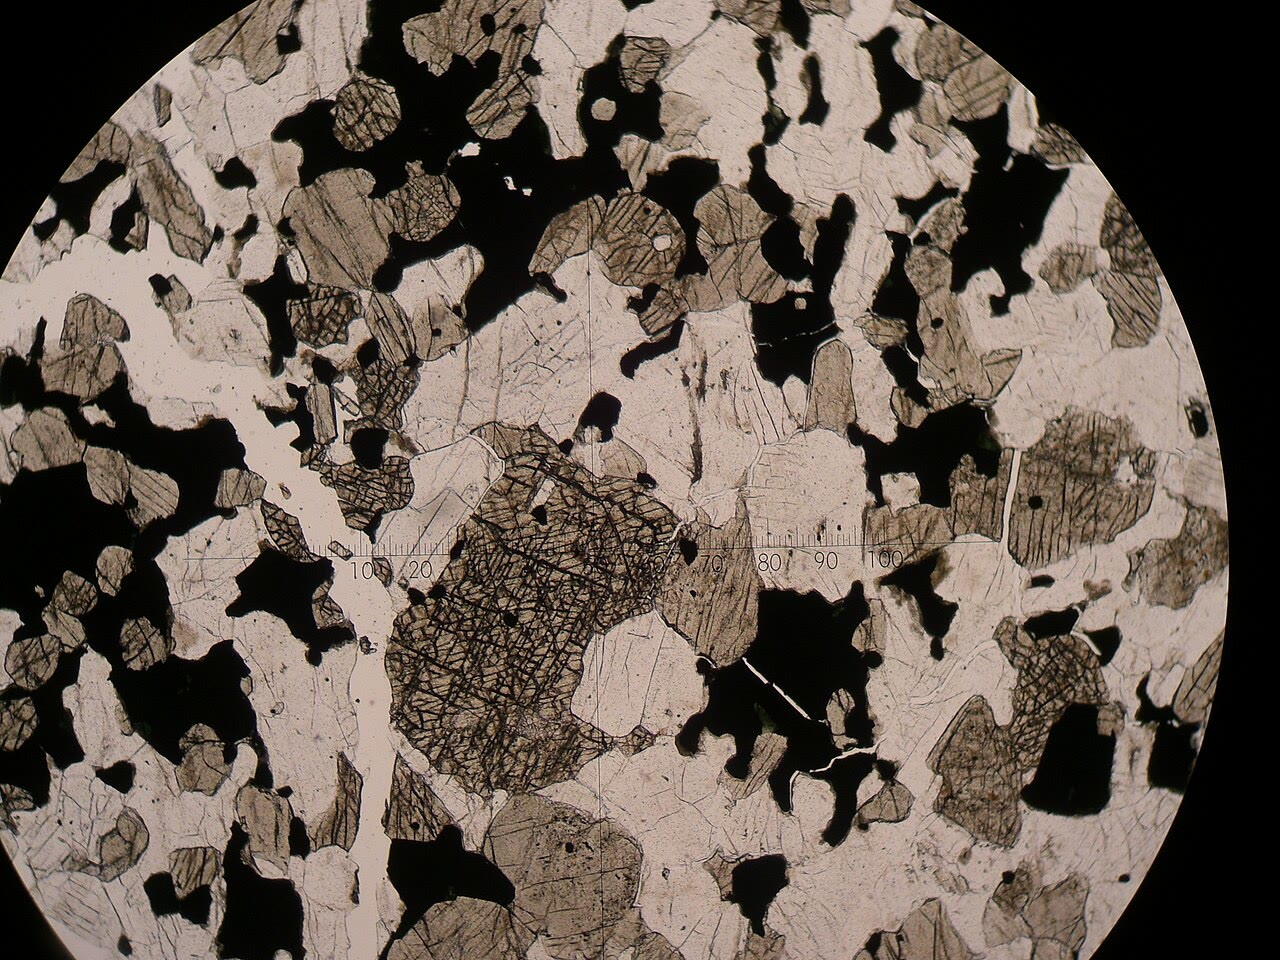
\includegraphics[width=0.485\linewidth]{images/book3/b1-gabbro-ppl.jpg} &
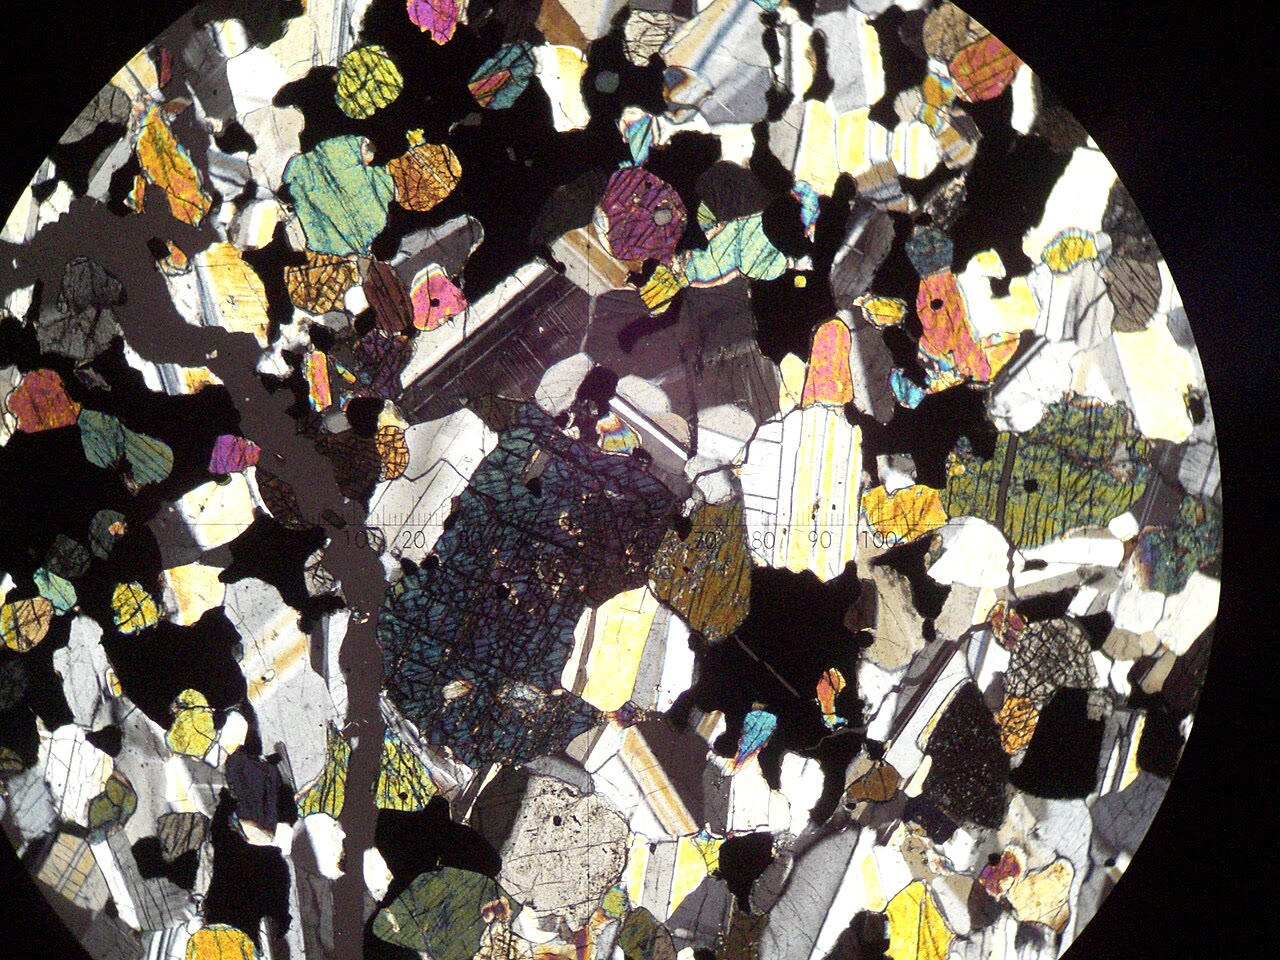
\includegraphics[width=0.485\linewidth]{images/book3/b1-gabbro-xpl.jpg} \\
{\small (a) \omterm{def:b1:field-lab-methods-1:microscope}{luz plano-polarizada}} & {\small (b) \omterm{def:b1:field-lab-methods-1:microscope}{polarizadores cruzados}} \\
\end{tabular}
% ledger: commons:gabbro-ppl, commons:gabbro-xpl

\medskip
{\small O mesmo campo de um gabro em \omterm{def:b1:field-lab-methods-1:thin-section}{lâmina delgada}. Em \omterm{def:b1:field-lab-methods-1:microscope}{luz plano-polarizada} (a), o \omterm{def:b1:rock-forming-minerals:groups}{plagioclásio} é incolor de \omterm{def:b1:optical-mineralogy:relief}{relevo} baixo, os grãos de \omterm{def:b1:rock-forming-minerals:groups}{piroxênio} e \omterm{def:b1:rock-forming-minerals:groups}{olivina} são cinza-marrom pálidos, de \omterm{def:b1:optical-mineralogy:relief}{relevo} alto e com fissuras densas, e o minério opaco é preto; a escala é um micrômetro na ocular. Entre \omterm{def:b1:field-lab-methods-1:microscope}{polarizadores cruzados} (b), as ripas de \omterm{def:b1:rock-forming-minerals:groups}{plagioclásio} são listradas pela \omterm{def:b1:optical-mineralogy:twin}{maclagem polissintética}, os grãos de \omterm{def:b1:rock-forming-minerals:groups}{piroxênio} e \omterm{def:b1:rock-forming-minerals:groups}{olivina} brilham em cores de segunda \omterm{def:b1:optical-mineralogy:interference-colour}{ordem}, e o minério permanece preto. Fotografias Chmee2, CC BY-SA 3.0 (Wikimedia Commons).}
\end{omfigure}

\begin{inthelab}[Uma sessão ao microscópio]
\begin{minipage}[t]{0.55\linewidth}\vspace{0pt}
Uma petróloga que descreve uma \omterm{def:b1:field-lab-methods-1:thin-section}{lâmina delgada} nova a percorre primeiro com pouco aumento, para ver a textura e os \omterm{def:b1:rock-forming-minerals:mineral}{minerais} principais, e depois grão a grão. Para cada \omterm{def:b1:rock-forming-minerals:mineral}{mineral} ela registra as observações do método acima, estima a sua proporção no campo e anota como os grãos se tocam: qual cristalizou primeiro, quais preenchem os espaços deixados, quais substituem outros. As medidas de luz são feitas com a platina graduada em graus e uma lâmina acessória; as composições, quando importam, são medidas depois com uma microssonda na mesma seção. Um laboratório de ensino funciona do mesmo modo, com um microscópio por estudante e uma caixa de lâminas de referência de \omterm{def:b1:rock-forming-minerals:mineral}{minerais} conhecidos ao lado.
\end{minipage}\hfill
\begin{minipage}[t]{0.42\linewidth}\vspace{0pt}
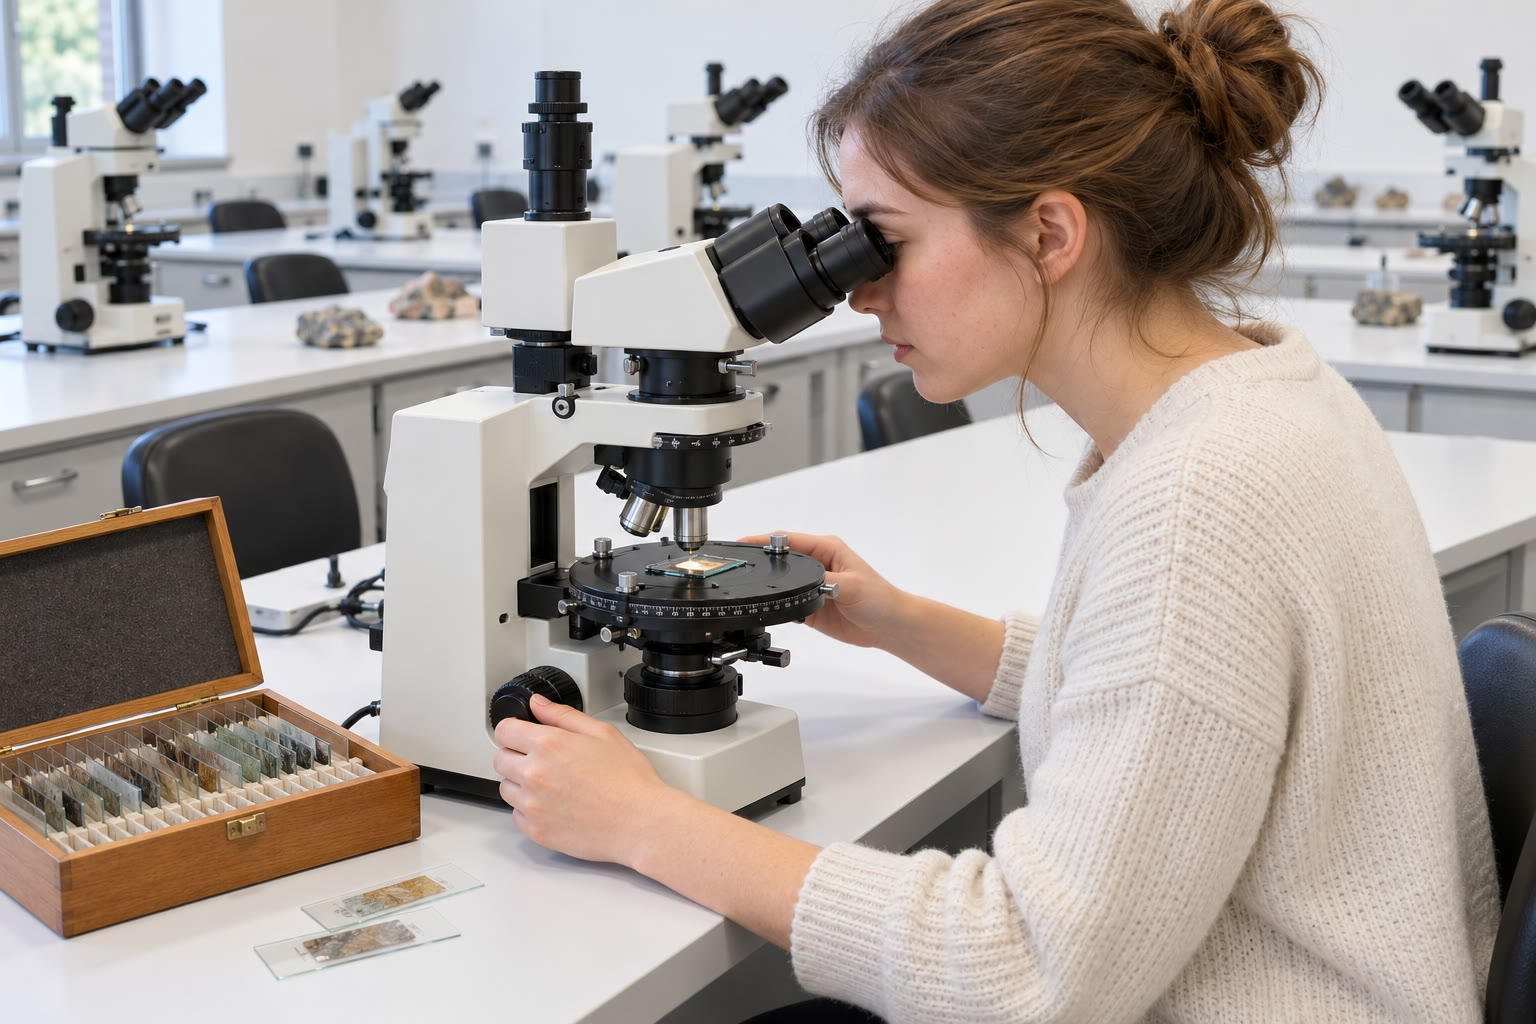
\includegraphics[width=\linewidth]{images/book3/ai/b1-microscope-student.jpg}

{\scriptsize Um estudante em um \omterm{def:b1:field-lab-methods-1:microscope}{microscópio de polarização} em um laboratório de ensino (ilustração gerada por IA).}
\end{minipage}
\end{inthelab}

\section{Exercícios}

\begin{exercise}[$\star$]\label{exo:b1:optical-mineralogy:1}
Calcule o \omterm{def:b1:optical-mineralogy:retardation}{retardo} máximo do quartzo ($\delta = 0.009$) e o da calcita ($\delta = 0.172$) em uma seção de \qty{30}{\micro m} de espessura. Usando a \omterm{def:b1:optical-mineralogy:interference-colour}{carta de Michel-Lévy}, descreva a cor de cada um.
% ledger: hom:quartz-optics, hom:calcite-optics
\end{exercise}

\begin{exercise}[$\star$]\label{exo:b1:optical-mineralogy:2}
Um grão é girado na platina entre \omterm{def:b1:field-lab-methods-1:microscope}{polarizadores cruzados}. Calcule $I/I_0$, como fração do seu máximo, em $\theta = 0$, \ang{22.5}, \ang{45}, \ang{67.5} e \ang{90} de uma \omterm{def:b1:optical-mineralogy:extinction}{posição de extinção}.
\end{exercise}

\begin{exercise}[$\star$]\label{exo:b1:optical-mineralogy:3}
Explique por que uma \omterm{def:b1:rock-forming-minerals:groups}{granada} permanece preta entre \omterm{def:b1:field-lab-methods-1:microscope}{polarizadores cruzados} qualquer que seja a posição da platina, e por que um grão de quartzo pode fazer o mesmo. Como você os distinguiria em \omterm{def:b1:field-lab-methods-1:microscope}{luz plano-polarizada}?
\end{exercise}

\begin{exercise}[$\star$]\label{exo:b1:optical-mineralogy:4}
Ordene por \omterm{def:b1:optical-mineralogy:relief}{relevo}, em um meio de índice $1.54$, ortoclásio ($n$ cerca de $1.52$), quartzo ($1.55$), forsterita ($1.65$) e almandina ($1.83$). Qual tem \omterm{def:b1:optical-mineralogy:relief}{relevo} negativo? Em que direção sua \omterm{def:b1:optical-mineralogy:relief}{linha de Becke} se desloca quando o foco é elevado?
% ledger: hom:orthoclase-optics, hom:quartz-optics, hom:forsterite-optics, hom:almandine-optics
\end{exercise}

\begin{exercise}[$\star\star$]\label{exo:b1:optical-mineralogy:5}
Em uma seção de \qty{30}{\micro m}, os grãos de um \omterm{def:b1:rock-forming-minerals:mineral}{mineral} verde \omterm{def:b1:optical-mineralogy:pleochroism}{pleocroico} com duas clivagens a \ang{56} e \ang{124} mostram no máximo um azul de segunda \omterm{def:b1:optical-mineralogy:interference-colour}{ordem}, lido na carta como $\Delta = \qty{650}{nm}$. Calcule a sua \omterm{def:b1:optical-mineralogy:birefringence}{birrefringência} e dê o nome do \omterm{def:b1:rock-forming-minerals:mineral}{mineral} com \cref{tab:b1:optical-mineralogy:key}.
\end{exercise}

\begin{exercise}[$\star\star$]\label{exo:b1:optical-mineralogy:6}
Usando \cref{prop:b1:optical-mineralogy:relief} com $n_m = 1.54$ e $i = \ang{30}$, calcule o desvio na borda de um grão de quartzo ($n = 1.553$) e de um grão de forsterita ($n = 1.651$), em graus, e a razão entre os dois. Confira a segunda com a lei de Snell exata.
\end{exercise}

\begin{exercise}[$\star\star$]\label{exo:b1:optical-mineralogy:7}
Uma lâmina vermelha de primeira \omterm{def:b1:optical-mineralogy:interference-colour}{ordem} tem $\Delta = \qty{540}{nm}$. Um grão de quartzo de $\Delta = \qty{270}{nm}$ é posto a \ang{45} com a lâmina inserida. Quais são os dois \omterm{def:b1:optical-mineralogy:retardation}{retardos} totais possíveis, e as cores que dão na carta? Qual orientação põe as duas direções lentas paralelas?
\end{exercise}

\begin{exercise}[$\star\star$]\label{exo:b1:optical-mineralogy:8}
Na sua borda afilada, um grão de fayalita ($\delta = 0.052$) se afina de \qty{30}{\micro m} até zero. Quantos matizes vermelho-violeta, que encerram as ordens em 542, 1074 e \qty{1605}{nm}, aparecem como franjas coloridas entre a borda e a parte de espessura total do grão?
% ledger: hom:fayalite-optics
\end{exercise}

\begin{exercise}[$\star\star$]\label{exo:b1:optical-mineralogy:9}
Em vários grãos alongados com uma boa clivagem, um geólogo mede \omterm{def:b1:optical-mineralogy:extinction}{ângulos de extinção} de \ang{0}, \ang{21}, \ang{36} e \ang{37} entre o traço da clivagem e a direção de vibração lenta. Por que os valores diferem? O \omterm{def:b1:rock-forming-minerals:mineral}{mineral} é mais provavelmente diopsídio ou hornblenda?
% ledger: hom:diopside-optics, hom:hornblende-optics
\end{exercise}

\begin{exercise}[$\star\star\star$]\label{exo:b1:optical-mineralogy:10}
Refaça a demonstração de \cref{thm:b1:optical-mineralogy:intensity} com o analisador paralelo ao polarizador, e mostre que
$I_\parallel = I_0\bigl(1 - \sin^2 2\theta\sin^2(\pi\Delta/\lambda)\bigr)$.
Que cor mostra um grão de $\Delta = \qty{550}{nm}$ a \ang{45} entre polarizadores paralelos?
\end{exercise}

\begin{exercise}[$\star\star\star$]\label{exo:b1:optical-mineralogy:11}
Para um grão de calcita com $\Delta = \qty{5000}{nm}$, o fator
$\sin^2(\pi\Delta/\lambda)$ se anula sempre que $\Delta/\lambda$ é um número inteiro. (a) Quantas vezes ele se anula entre \num{400} e \qty{700}{nm}? (b) Mostre que, perto de $\lambda = \qty{550}{nm}$, dois zeros sucessivos distam cerca de $\lambda^2/\Delta$, e calcule. (c) Explique por que o grão parece quase branco.
\end{exercise}

\begin{exercise}[$\star\star\star$]\label{exo:b1:optical-mineralogy:12}
Mostre que, em média sobre uma volta completa da platina, um grão entre \omterm{def:b1:field-lab-methods-1:microscope}{polarizadores cruzados} transmite $\frac12 I_0\sin^2(\pi\Delta/\lambda)$. Um geólogo estima \omterm{def:b1:optical-mineralogy:birefringence}{birrefringências} a partir da cor mais alta de cada \omterm{def:b1:rock-forming-minerals:mineral}{mineral}, supondo \qty{30}{\micro m}, em uma seção que na verdade tem \qty{25}{\micro m} de espessura. Por que fator todos os seus valores estão errados, e em que sentido?
\end{exercise}

\section{Problema: identificando os minerais de uma lâmina desconhecida}

\begin{problem}[{Problema de fim de semana --- observando relevo, pleocroísmo e cores de interferência, medindo a espessura de uma seção com quartzo, e dando nome a seus minerais}]
\label{pb:b1:optical-mineralogy:1}
% values: calc/ch08.py; optical data: ledger hom:*-optics
% ledger: hom:quartz-optics, hom:diopside-optics, hom:forsterite-optics, hom:albite-optics, hom:anorthite-optics, hom:hornblende-optics, hom:biotite-optics
Uma \omterm{def:b1:field-lab-methods-1:thin-section}{lâmina delgada} de uma rocha ígnea desconhecida, montada em uma resina de índice
$1.540$, tem espessura de \qty{30}{\micro m}, segundo se diz. Contém cinco \omterm{def:b1:rock-forming-minerals:mineral}{minerais}, rotulados de A a E. Use a tabela de propriedades ópticas do capítulo, a \omterm{def:b1:optical-mineralogy:interference-colour}{carta de Michel-Lévy} e os seguintes valores: quartzo $n_\omega = 1.544$,
$n_\varepsilon = 1.553$; diopsídio $n_\alpha = 1.664$, $n_\beta = 1.672$,
$n_\gamma = 1.694$.

\medskip
\noindent\textbf{Parte I --- Luz plano-polarizada.}
\begin{enumerate}
  \item O \omterm{def:b1:rock-forming-minerals:mineral}{mineral} A é incolor, com bordas de grãos difíceis de ver. O \omterm{def:b1:rock-forming-minerals:mineral}{mineral} B é incolor, com bordas escuras fortes e duas clivagens que se encontram a cerca de \ang{87}. Qual tem o \omterm{def:b1:optical-mineralogy:relief}{relevo} mais alto?
  \item Para A, tomado como quartzo, e B, tomado como diopsídio, calcule $|n - n_m|$ usando a média dos índices principais de cada um.
  \item Usando \cref{prop:b1:optical-mineralogy:relief}, calcule a razão entre os desvios nas bordas dos dois, para a mesma inclinação da fronteira.
  \item Ao elevar o foco, a \omterm{def:b1:optical-mineralogy:relief}{linha de Becke} de B se desloca para dentro do grão. O que isso mostra?
  \item O \omterm{def:b1:rock-forming-minerals:mineral}{mineral} C vai de amarelo pálido a marrom escuro à medida que a platina gira, mais escuro quando sua única clivagem fica ao longo do polarizador. Dê o nome da propriedade e do \omterm{def:b1:rock-forming-minerals:mineral}{mineral}.
  \item O \omterm{def:b1:rock-forming-minerals:mineral}{mineral} D é incolor, de \omterm{def:b1:optical-mineralogy:relief}{relevo} baixo, em ripas longas; E é verde a amarelo e \omterm{def:b1:optical-mineralogy:pleochroism}{pleocroico}, com duas clivagens a \ang{124}. O que o ângulo sugere para E?
\end{enumerate}

\medskip
\noindent\textbf{Parte II --- A espessura da seção.}
\begin{enumerate}[resume]
  \item Qual é o maior \omterm{def:b1:optical-mineralogy:retardation}{retardo} do quartzo em uma seção de exatamente \qty{30}{\micro m}? Qual é a sua cor?
  \item Por que o maior \omterm{def:b1:optical-mineralogy:retardation}{retardo} deve ser procurado entre muitos grãos de A, em vez de medido em um só deles?
  \item A cor mais alta mostrada pelos grãos de A é um amarelo pálido de primeira \omterm{def:b1:optical-mineralogy:interference-colour}{ordem}; um comparador de cunha de quartzo dá o seu \omterm{def:b1:optical-mineralogy:retardation}{retardo} como \qty{342}{nm}. Calcule a espessura real da seção.
  \item De quantos por cento a seção é mais espessa do que deveria ser?
  \item Em $\lambda = \qty{550}{nm}$ e a \ang{45} da extinção, calcule $I/I_0$ para esse grão de quartzo, e para o mesmo grão em uma seção de \qty{30}{\micro m}.
  \item Calcule a faixa de \omterm{def:b1:optical-mineralogy:retardation}{retardos} de D, tomado como \omterm{def:b1:rock-forming-minerals:groups}{plagioclásio} ($\delta = 0.008$ a $0.013$), nesta seção, e diga se suas cores permanecem na primeira \omterm{def:b1:optical-mineralogy:interference-colour}{ordem}.
\end{enumerate}

\medskip
\noindent\textbf{Parte III --- A birrefringência de B.}
\begin{enumerate}[resume]
  \item A cor mais alta de B é um azul lido como $\Delta = \qty{1140}{nm}$. Em qual \omterm{def:b1:optical-mineralogy:interference-colour}{ordem} ela está?
  \item Calcule a \omterm{def:b1:optical-mineralogy:birefringence}{birrefringência} de B com a espessura encontrada na questão 9.
  \item Que \omterm{def:b1:optical-mineralogy:birefringence}{birrefringência} se teria encontrado supondo \qty{30}{\micro m}? Que \omterm{def:b1:rock-forming-minerals:mineral}{mineral} incolor de \omterm{def:b1:optical-mineralogy:relief}{relevo} alto isso teria sugerido, e por que ele está deslocado em uma rocha com quartzo (considere \ce{Mg2SiO4 + SiO2 -> 2 MgSiO3})?
  \item Compare o resultado da questão 14 com a tabela, junto com o \omterm{def:b1:optical-mineralogy:relief}{relevo} e as clivagens de B, e conclua.
  \item Que cor B mostraria no máximo em uma seção correta de \qty{30}{\micro m}?
  \item A seção é desbastada até \qty{30}{\micro m}. Quanto deve ser afinada, e qual é então a cor mais alta do quartzo?
\end{enumerate}

\medskip
\noindent\textbf{Parte IV --- Extinção e maclagem.}
\begin{enumerate}[resume]
  \item As ripas de D são divididas em listras paralelas que se extinguem alternadamente. Dê o nome da feição e do \omterm{def:b1:rock-forming-minerals:mineral}{mineral}.
  \item As listras de uma ripa se extinguem a \ang{27} e \ang{28} de cada lado do plano de \omterm{def:b1:optical-mineralogy:twin}{macla}. Que composição indicam esses ângulos, medidos em muitas ripas, quando comparados com cartas publicadas?
  \item O maior \omterm{def:b1:optical-mineralogy:extinction}{ângulo de extinção} entre as clivagens de E e sua direção lenta é \ang{17}. Dê o nome de E.
  \item Calcule o maior \omterm{def:b1:optical-mineralogy:retardation}{retardo} de E nesta seção e a cor que ele mostra.
  \item Um grão de B permanece escuro durante uma volta completa. Explique como ele pode ser o mesmo \omterm{def:b1:rock-forming-minerals:mineral}{mineral} dos grãos brilhantes de B.
  \item Liste os \omterm{def:b1:rock-forming-minerals:mineral}{minerais} A a E e diga que tipo de rocha eles formam.
  \item Qual é a espessura real da seção, em micrômetros?
\end{enumerate}
\end{problem}
